\chapter{Análisis de resultados}
\section{Análisis de la última temporada}
Vamos a comenzar analizando cómo varían las distintas tasas de aciertos entre las jornadas 21 y 38 de la temporada 2014/15 para los modelos propuestos. Para ello extraemos los datos usando varios scripts automatizados que obtienen la predicción (ya sea de partidos o de rankings) y los compara con los resultados reales.

\subsection{Modelo basado en la posición relativa}
En la siguiente gráfica se muestra el número de partidos acertados (de los 10 que se disputan) en cada jornada usando el modelo de interpolación.
\begin{figure}[H]
	\centering
	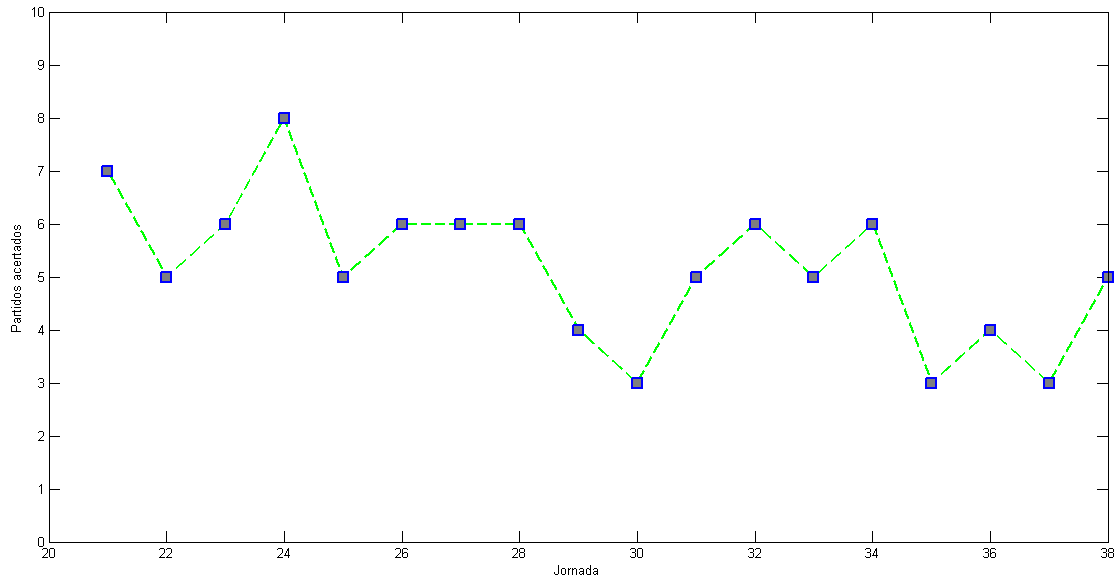
\includegraphics[scale=0.45]{images/aciertos_partidos_modelo1.png}
	\caption{Interpolación: Número de partidos acertados.}
\end{figure}

Ahora analizaremos la tasa de aciertos en la predicción de la clasificación. Recordemos del capítulo anterior que usábamos tres formas para realizar esta tarea: comparar que los rankings coinciden posición por posición, la Tau de Kendall y la Rho de Spearman. El problema de la Rho de Spearman es que no está acotada por lo que no nos va a aportar tanta información como los gráficos de las otras alternativas, por ello decidimos no usarla. Al comparar posición por posición predecir mal un solo partido puede descolocar bastantes posiciones cuando la diferencia entre ellas es de pocos puntos. La medida que más nos interesa estudiar es la Tau de Kendall, que analiza el número de pares de equipos cuya posición relativa en ambos rankings es la misma, su valor está entre $-1$ y $1$, siendo más similares cuanto más se aproximen a 1.\\

En la siguiente gráfica se muestra el número de posiciones correctas (de las 20 del ranking) en cada jornada usando el modelo de interpolación.
\begin{figure}[H]
	\centering
	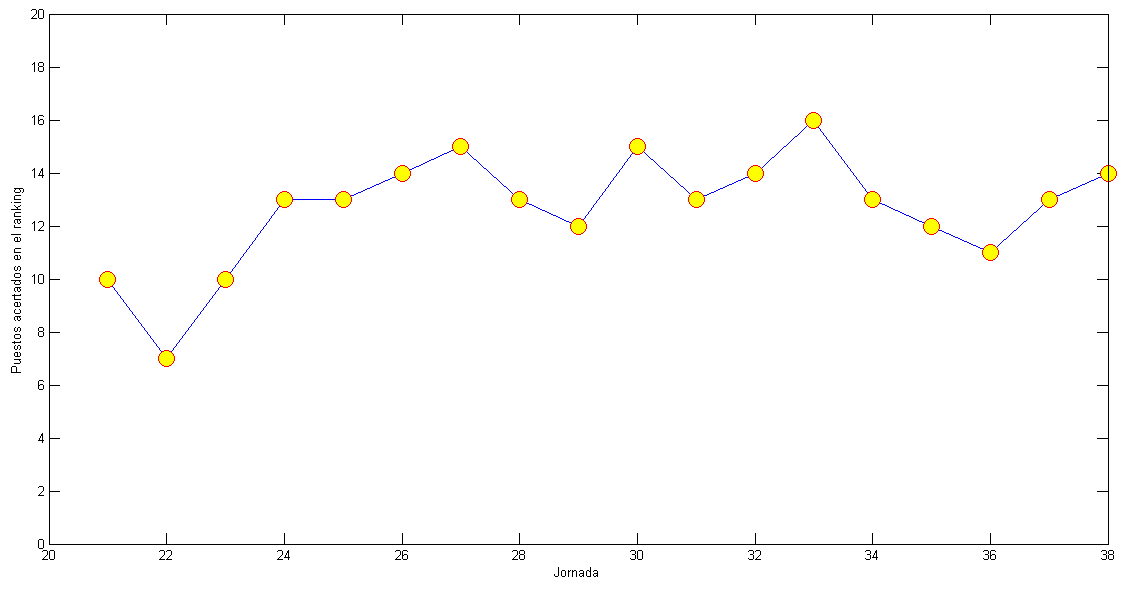
\includegraphics[scale=0.45]{images/aciertos_ranking_modelo1.png}
	\caption{Interpolación: Número de posiciones del ranking acertadas.}
\end{figure}

Y a continuación se muestra la evolución de la Tau de Kendall a lo largo de las jornadas usando el modelo de interpolación.
\begin{figure}[H]
	\centering
	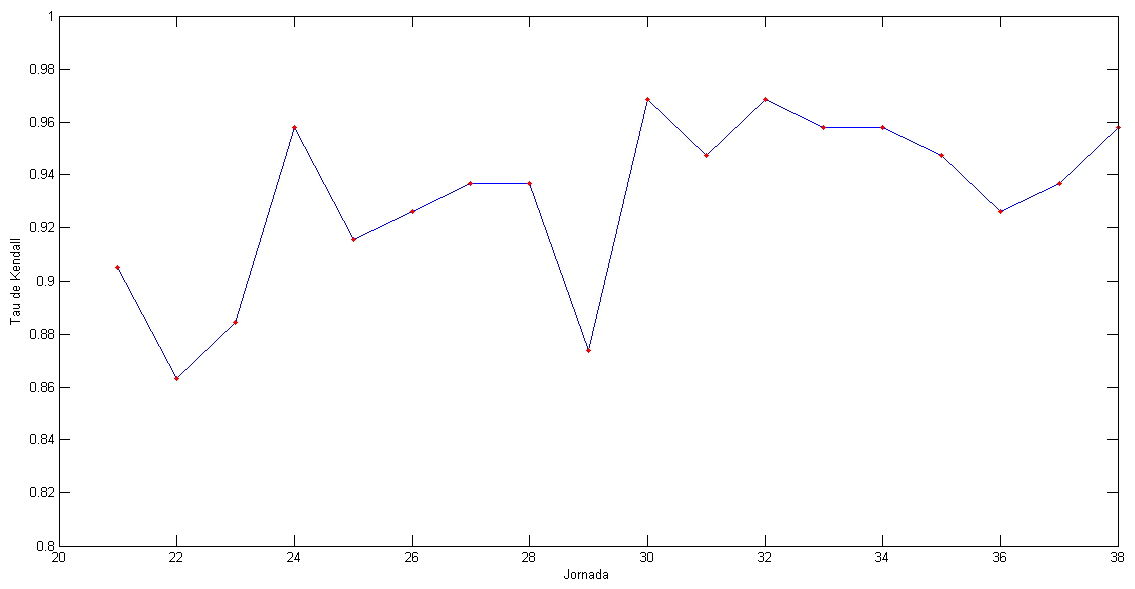
\includegraphics[scale=0.45]{images/tau_modelo1.png}
	\caption{Interpolación: Evolución de la Tau de Kendall.}
\end{figure}

\subsection{Modelo basado en la tendencia de los equipos}
En las gráficas de esta sección siempre aparecerán tres funciones, que se corresponden con la función memoria (constante, lineal o exponencial) seleccionada para el modelo de tendencias.\\

De nuevo, la primera gráfica muestra el número de partidos acertados (de los 10 que se disputan), en la segunda el número de posiciones correctas (de las 20 del ranking) y en la última la evolución de la Tau de Kendall a lo largo de las jornadas usando el modelo de tendencias de los equipos.
\begin{figure}[H]
	\centering
	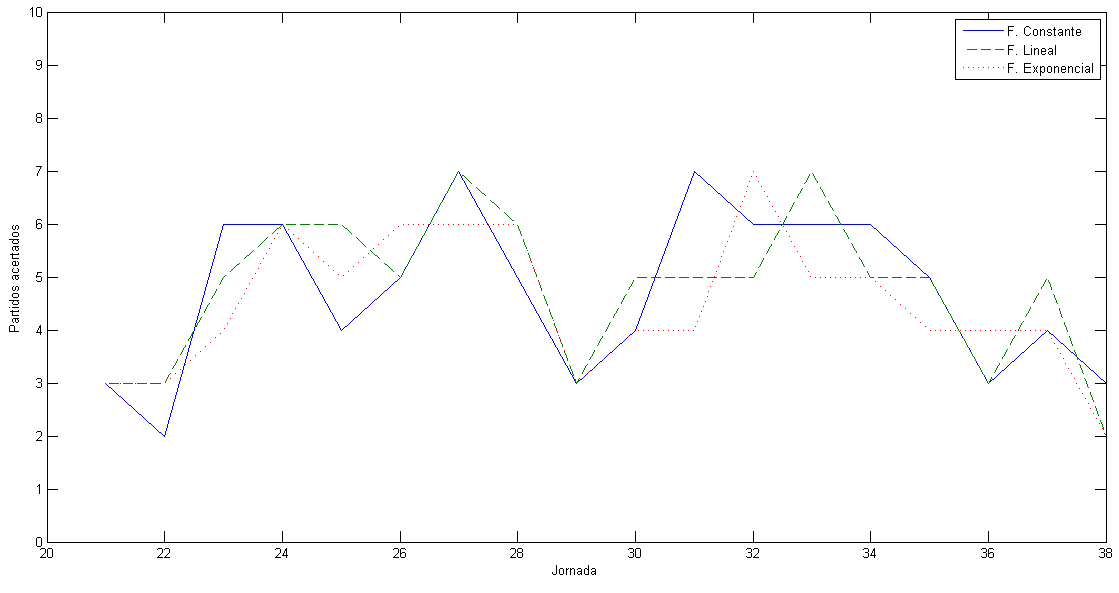
\includegraphics[scale=0.5]{images/aciertos_partidos_modelo2.png}
	\caption{Tendencias: Número de partidos acertados.}
\end{figure}

\begin{figure}[H]
	\centering
	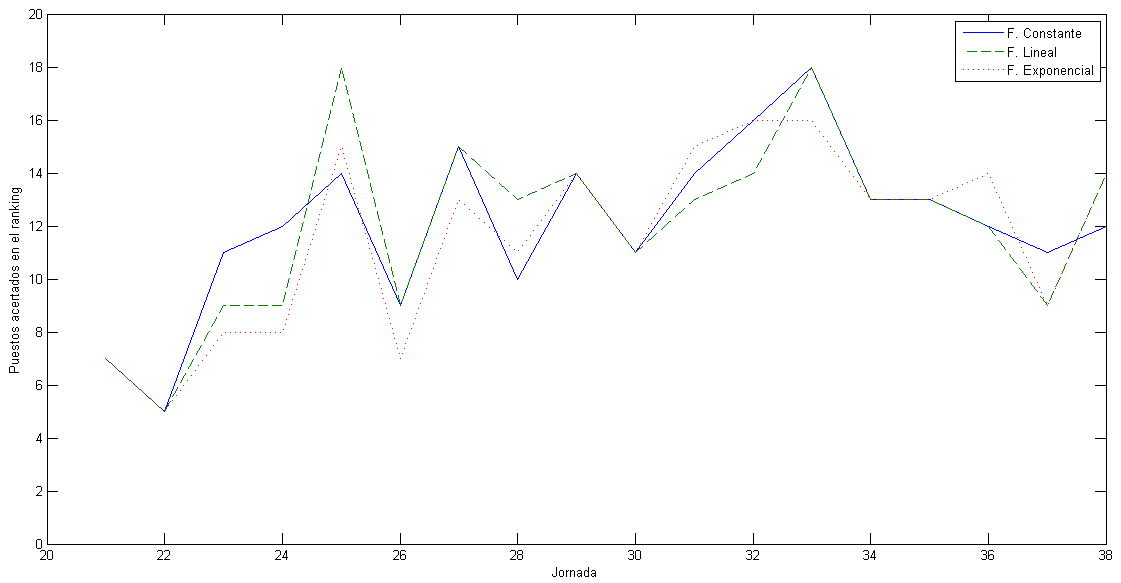
\includegraphics[scale=0.5]{images/aciertos_ranking_modelo2.png}
	\caption{Tendencias: Número de posiciones del ranking acertadas.}
\end{figure}

\begin{figure}[H]
	\centering
	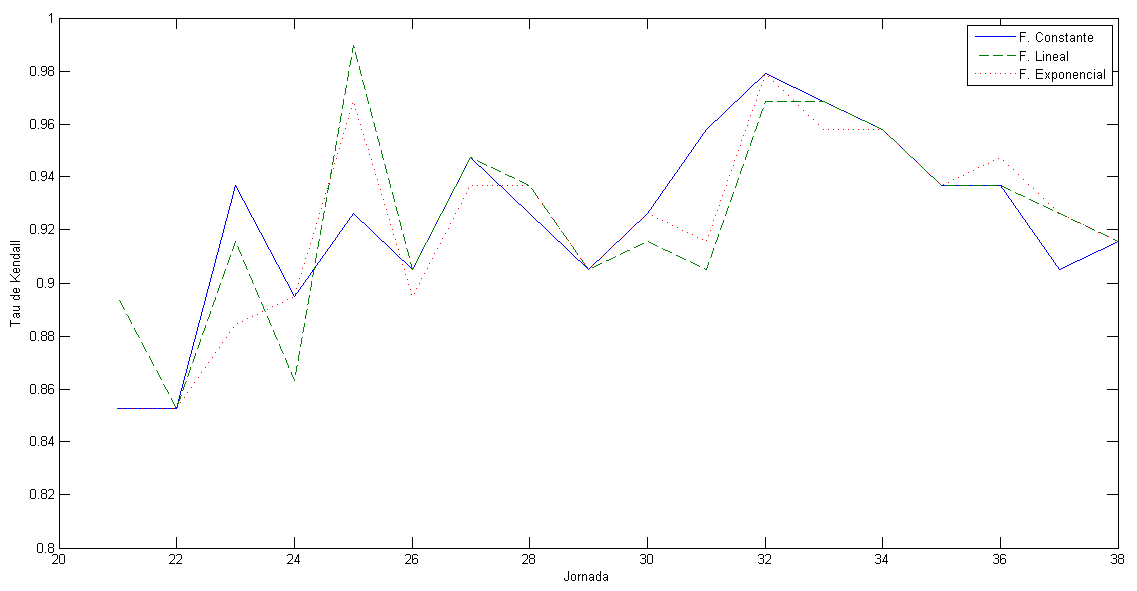
\includegraphics[scale=0.5]{images/tau_modelo2.png}
	\caption{Tendencias: Evolución de la Tau de Kendall.}
\end{figure}
En las gráficas de la figura \ref{fig:comparacion_func} analizamos cuál de las tres funciones nos da mejores resultados, el número total de aciertos de los partidos del modelo lineal son 86, del constante 85 y del exponencial 81. Por tanto, la mejor función memoria para esta temporada es el resultante de aplicar la función memoria lineal.
\begin{figure}[H]
	\centering
	\subfloat[Partidos]{
		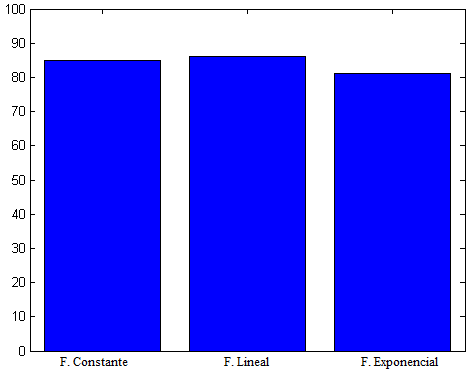
\includegraphics[width=0.5\textwidth]{images/comp_func_mem_1_partidos.png}}
	\subfloat[Ranking]{
		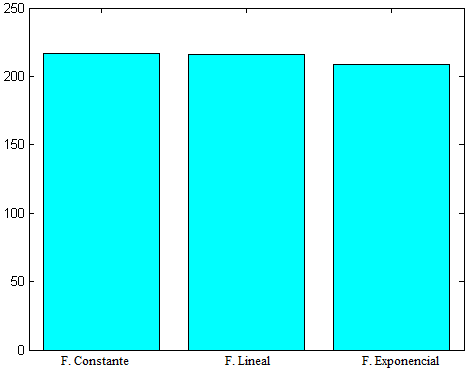
\includegraphics[width=0.5\textwidth]{images/comp_func_mem_1_ranking.png}}	
	\caption{Tendencias: Comparación de las tres funciones memoria.} \label{fig:comparacion_func}
\end{figure} 

\newpage

\subsection{Combinación de los modelos}
En la siguiente gráfica se muestra el número total de partidos que se acertarían (de los 180 que se disputan en las 18 jornadas) dependiendo del valor que tome $\lambda$.
\begin{figure}[H]
	\centering
	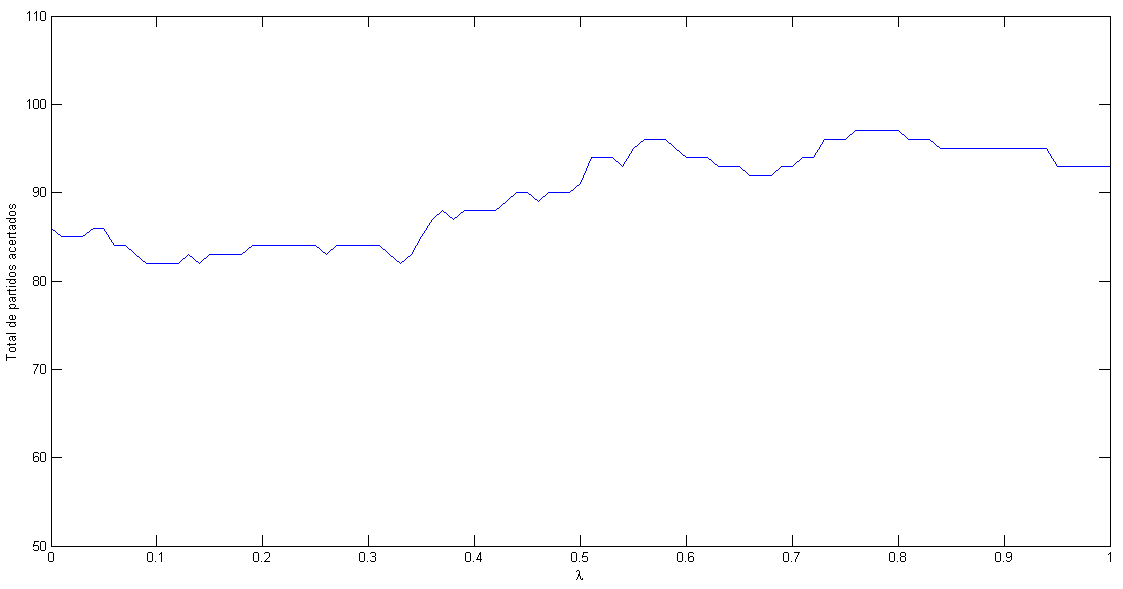
\includegraphics[scale=0.5]{images/aciertos_partidos_modelo3.png}
	\caption{Combinación: Evolución de $\lambda$.} \label{fig:evol_lambda}
\end{figure}

En las siguientes gráficas se muestra el número de posiciones correctas (de las 20 del ranking) y la evolución de la Tau de Kendall a lo largo de las jornadas usando el modelo de combinación con $\lambda \in [0.76,0.80]$.
\begin{figure}[H]
	\centering
	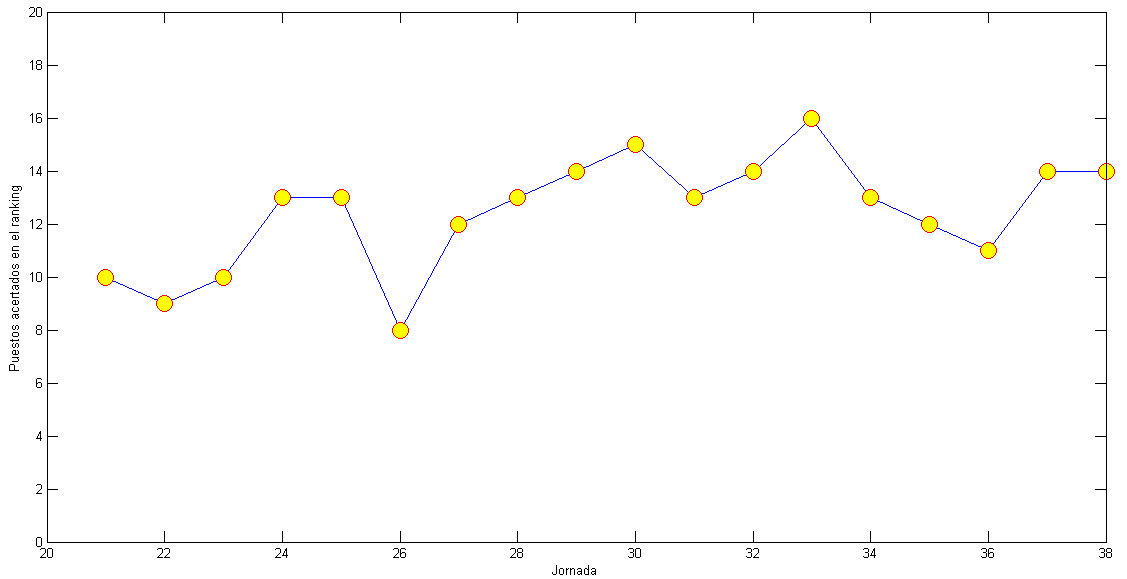
\includegraphics[scale=0.5]{images/aciertos_ranking_modelo3.png}
	\caption{Combinación: Número de posiciones del ranking acertadas.}
\end{figure}
 
\begin{figure}[H]
	\centering
	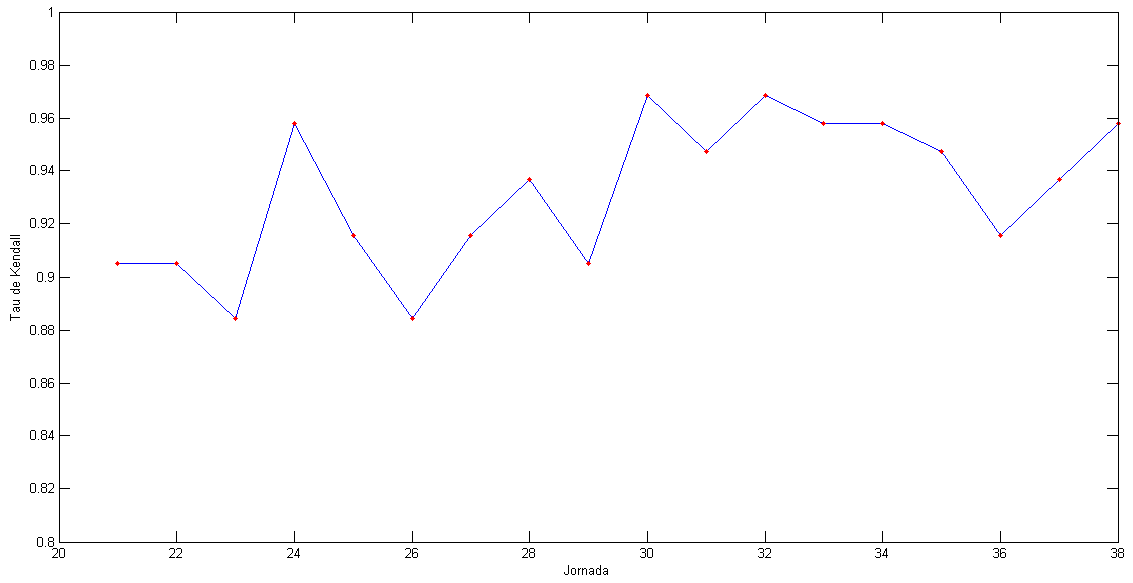
\includegraphics[scale=0.5]{images/tau_modelo3.png}
	\caption{Combinación: Evolución de la Tau de Kendall.}
\end{figure}

\ \\

\newpage

\subsection{Resultados}
Finalmente vamos a comparar el número de predicciones correctas que realiza cada uno de nuestros modelos. Las gráficas en las que se comparan el número de aciertos del total de partidos de la temporada, del total de posiciones del ranking y el valor medio de la Tau de Kendall se puede encontrar en la figura \ref{fig:comparacion_modelos}.\\

\begin{figure}[H]
	\centering
	\subfloat[Partidos]{
		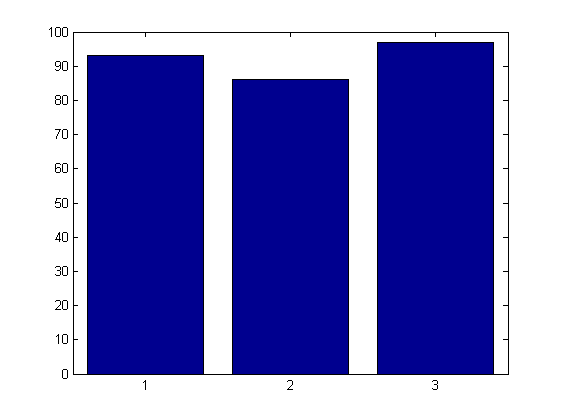
\includegraphics[width=0.45\textwidth]{images/comp_mod_partidos.png}}\\
	\subfloat[Ranking]{
		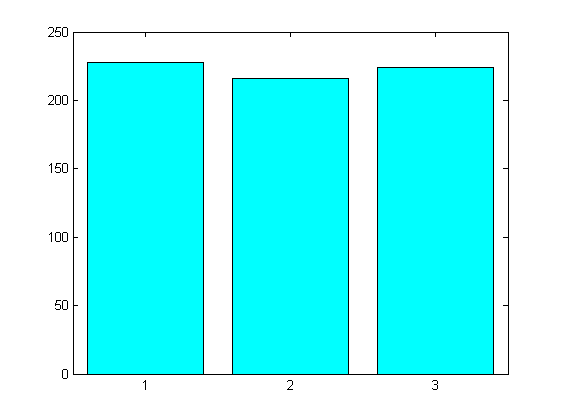
\includegraphics[width=0.45\textwidth]{images/comp_mod_ranking.png}}	
	\subfloat[Tau de Kendall]{
		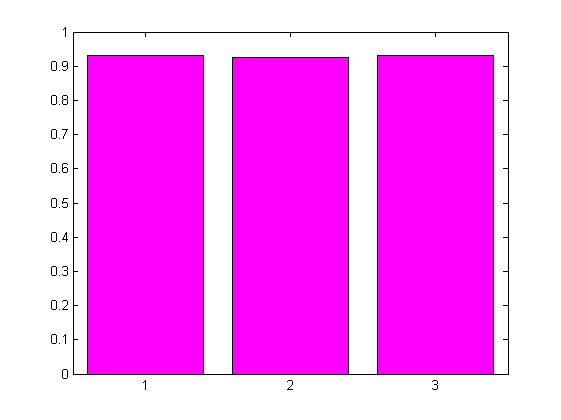
\includegraphics[width=0.45\textwidth]{images/comp_mod_tau.png}}	
	\caption{Comparación de los tres modelos propuestos.} \label{fig:comparacion_modelos}
\end{figure} 

El modelo de combinación es con el que se acierta el mayor número de partidos, acertando un total de 97, lo que claramente aumenta los aciertos que se obtienen usando cada método por separado, 93 en el caso del modelo basado en la posición relativa y 86 en el caso del basado en la tendencia de los equipos. \\

Sin embargo, si lo que comparamos es el valor medio de la Tau de Kendall para ver la tasa de aciertos en la predicción de rankings, el modelo basado en la posición relativa y el modelo de la combinación obtienen exactamente el mismo valor, $\tau=0.9315789$.\\ 

\section{Comparación con otras temporadas}
En esta sección vamos a comparar los resultados obtenidos de la temporada 2014-2015 con los de temporadas anteriores, concretamente la 2012-2013 y la 2013-2014.

\subsection{Modelo basado en la posición relativa}
En los siguientes gráficos se muestran, respectivamente, el número total de aciertos de partidos, de los rankings (posición a posición) y la media de la Tau de Kendall para las últimas tres temporadas usando el modelo de interpolación.

\begin{figure}[H]
	\centering
	\subfloat[Partidos]{
		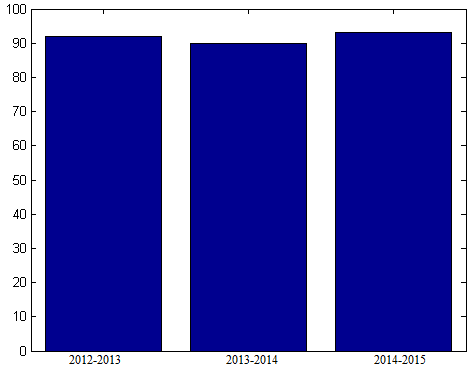
\includegraphics[width=0.5\textwidth]{images/comp_temp_mod1_part.png}}\\
	\subfloat[Ranking]{
		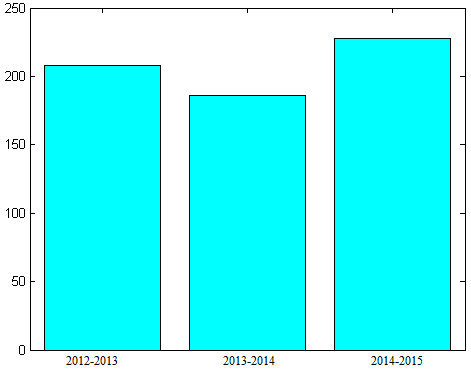
\includegraphics[width=0.5\textwidth]{images/comp_temp_mod1_rank.png}}	
	\subfloat[Tau de Kendall]{
		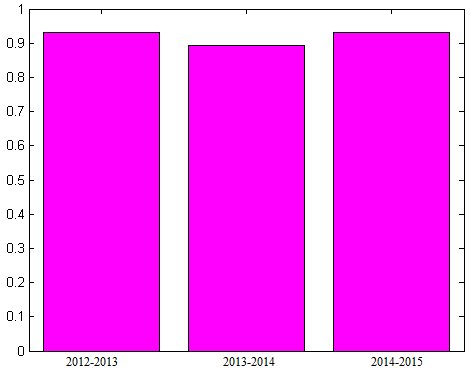
\includegraphics[width=0.5\textwidth]{images/comp_temp_mod1_tau.png}}
	\caption{Interpolación: Comparación de las últimas temporadas.}
\end{figure}

\subsection{Modelo basado en la tendencia de los equipos}
En los siguientes gráficos se muestran, respectivamente, el número total de aciertos de partidos, de los rankings (posición a posición) y la media de la Tau de Kendall para las últimas tres temporadas usando el modelo de tendencias.
\begin{figure}[H]
	\centering
	\subfloat[Partidos]{
		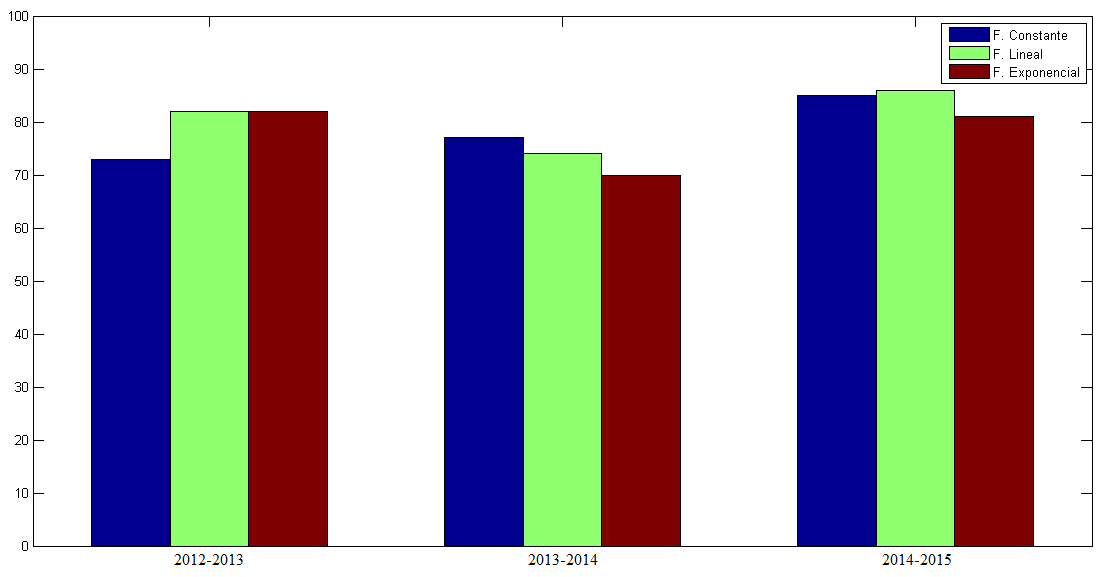
\includegraphics[width=0.63\textwidth]{images/comp_temp_mod2_mem_part.png}}\\
	\subfloat[Ranking]{
		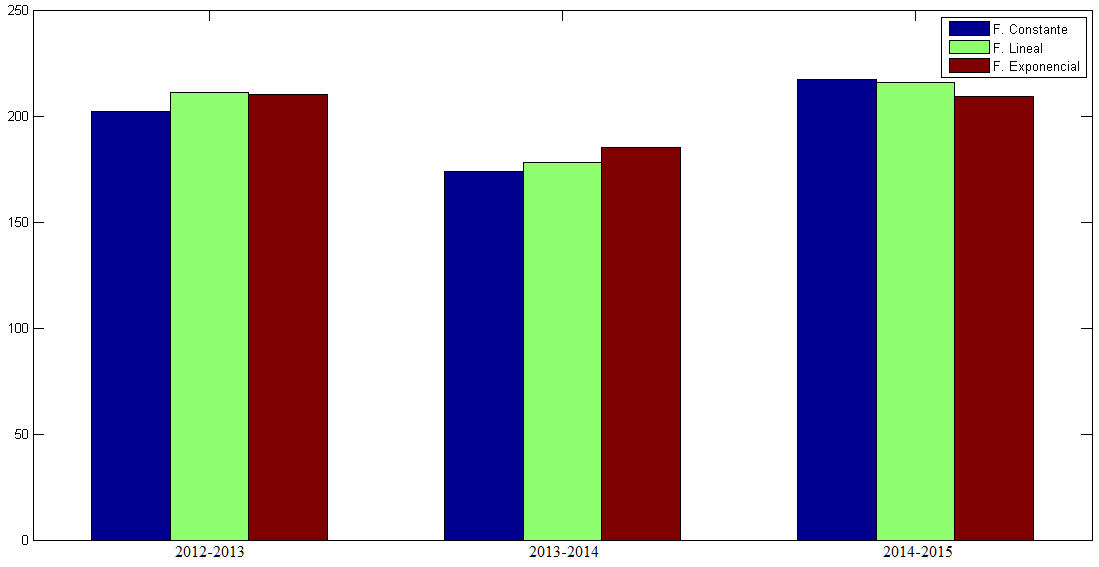
\includegraphics[width=0.63\textwidth]{images/comp_temp_mod2_mem_rank.png}}\\	
	\subfloat[Tau de Kendall]{
		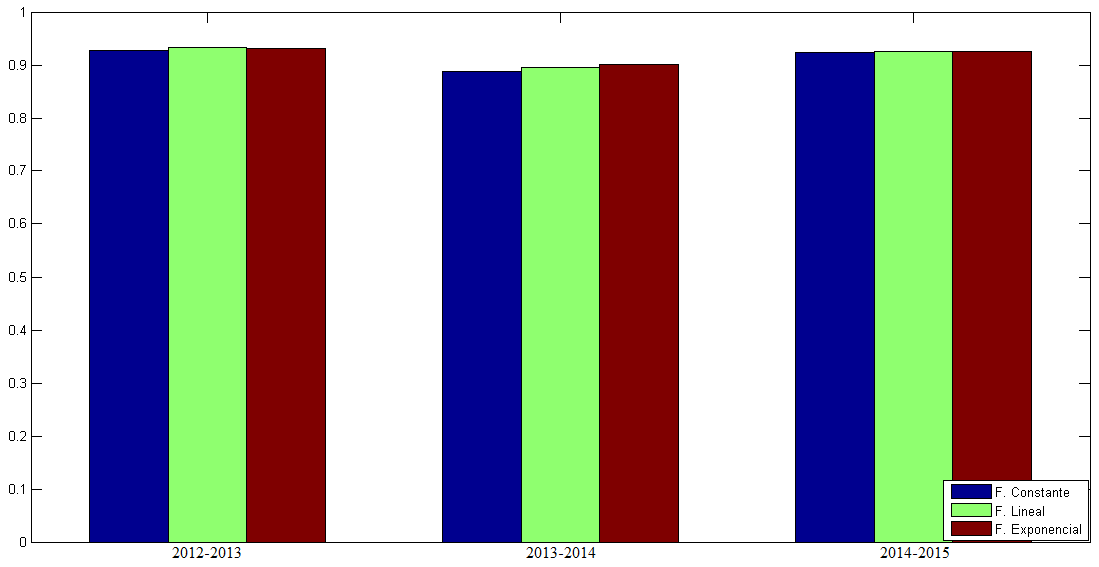
\includegraphics[width=0.63\textwidth]{images/comp_temp_mod2_mem_tau.png}}
	\caption{Tendencias: Comparación de las funciones memoria de las últimas temporadas.}
\end{figure}

Analizando las gráficas anteriores obtenemos la siguiente tabla. En ella elegimos la mejor función memoria teniendo en cuenta la temporada y si la predicción la estamos haciendo de partidos o de la clasificación.

\begin{center}
	\begin{tabular}{|c|c|c|c|}
		\hline &  2012/13 &  2013/14 &  2014/15 \\ 
		\hline Partidos & Lineal/Exponencial &  Constante &  Lineal \\ 
		\hline Ranking  &  Lineal &  Exponencial &  Constante \\ 
		\hline 
	\end{tabular} 
\end{center}

\subsection{Combinación de los modelos}
En la siguiente figura se muestran los valores que debe tomar lambda en las últimas tres temporadas para obtener el mayor número de aciertos.

\begin{figure}[H]
	\centering
	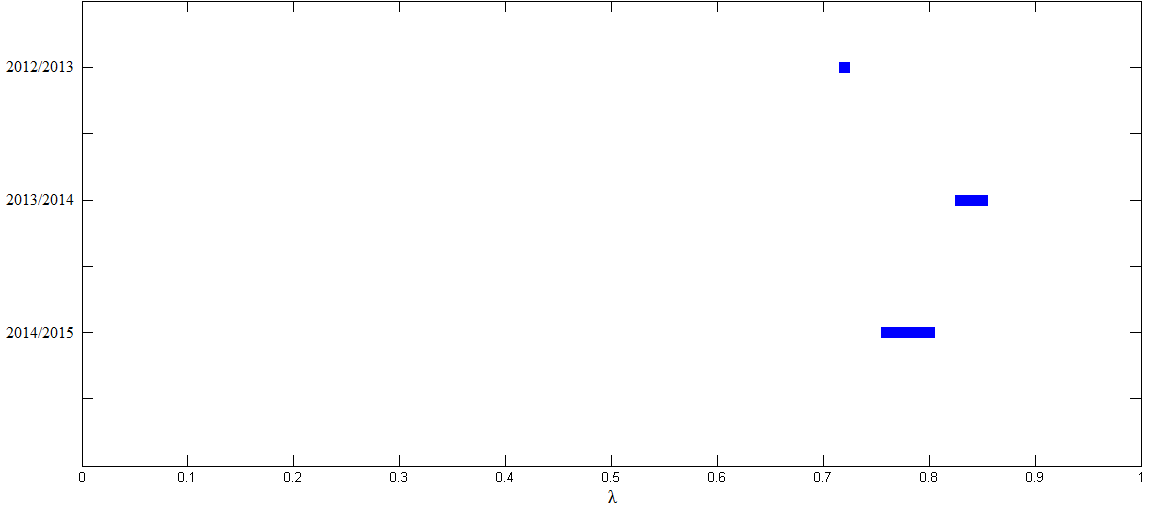
\includegraphics[scale=0.57]{images/comp_temp_mod3_lambda.png}
	\caption{Combinación: Valores óptimos de $\lambda$ de las últimas temporadas.} \label{fig:lambda_temp}
\end{figure}

En la temporada 2012/13 solo hay un valor óptimo de $\lambda$ que es $0.72$ mientras que para las otras dos hay un intervalo de valores óptimos, respectivamente $\lambda \in [0.83,0.85]$ para la 2013/14 y $\lambda \in [0.76,0.80]$ para la 2014/15.\\

Como ya vimos en la figura \ref{fig:evol_lambda}, el modelo de combinación suele obtener mayor número de aciertos cuando $\lambda$ oscila entre los valores $0.7$ y $0.9$. Y acabamos de ver en la figura \ref{fig:lambda_temp} que para el resto de temporadas analizadas se cumple que $\lambda$ oscila entre dichos valores. \\

En los siguientes gráficos se muestran, respectivamente, el número total de aciertos de partidos, de los rankings (posición a posición) y la media de la Tau de Kendall para las últimas tres temporadas usando la combinación de modelos, cada uno con su valor óptimo de $\lambda$.

\begin{figure}[H]
	\centering
	\subfloat[Partidos]{
		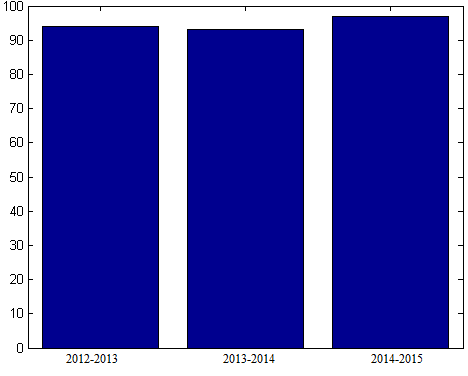
\includegraphics[width=0.5\textwidth]{images/comp_temp_mod3_part.png}}\\
	\subfloat[Ranking]{
		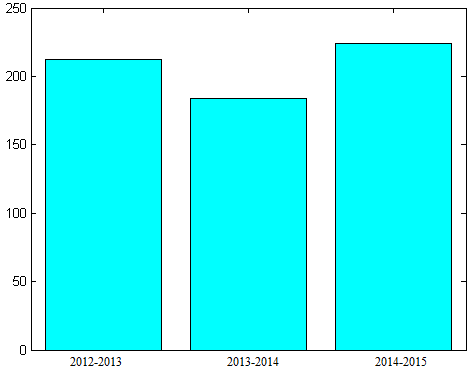
\includegraphics[width=0.5\textwidth]{images/comp_temp_mod3_rank.png}}	
	\subfloat[Tau de Kendall]{
		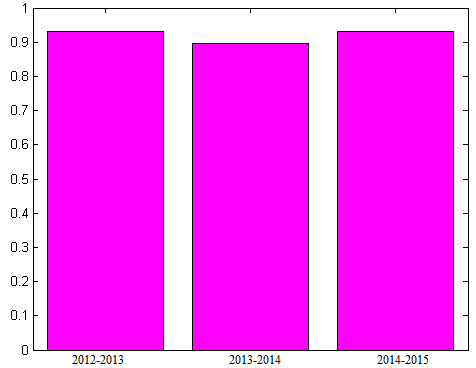
\includegraphics[width=0.5\textwidth]{images/comp_temp_mod3_tau.png}}
	\caption{Combinación: Comparación de las últimas temporadas.}
\end{figure} 

\newpage
\subsection{Resultados}
Las conclusiones de todos los resultados mostrados que se pueden sacar son:
\begin{itemize}
	\item El modelo basado en la tendencia de los equipos es algo inferior a los otros dos modelos propuestos independientemente de la función memoria que usemos. 
	\item Las variaciones entre usar una función memoria u otra en el modelo basado en la tendencia de los equipos no son significativas. Dependiendo de la temporada y de si lo que queremos predecir con mayor tasa de aciertos son los partidos o las posiciones en la clasificación, la mejor función memoria con respecto a las otras cambia.  
	\item La combinación de los dos modelos es el que obtiene mayor número de aciertos en las predicciones de los partidos. Aunque en la predicción de la clasificación la media de la Tau de Kendall suele ser muy similar a la del modelo basado en la posición relativa de los equipos.
	\item El valor óptimo de $\lambda$ en la combinación de modelos siempre suele oscilar entre $\lambda=0.7$ y $\lambda=0.9$. Es decir, $\lambda$ ``da más peso'' a los resultados del modelo de interpolación que al modelo de tendencias a la hora de combinarlos, lo que es lógico porque, como ya hemos indicado, el modelo de interpolación es bastante superior al de tendencias.
	\item A medida que avanzan las temporadas, se van obteniendo umbrales más fiables para aplicarlos en el modelo de interpolación, lo que provoca que poco a poco se vaya incrementando el número de partidos acertados.
	\item El número de aciertos total de los modelos de interpolación y el modelo combinatorio suele estar por encima de los 90 aciertos pero por debajo de los 100 (del total de 180 partidos que se predicen cada temporada, 10 partidos $x$ 18 jornadas) lo que quiere decir que suelen acertar en torno al $50-55\%$ de los partidos. El porcentaje es bastante inferior, en torno al $40-45\%$, en el modelo de tendencias. Porcentajes que no están nada mal y superiores a métodos como el de selección aleatoria ($33\%$) o el método de elección de victoria local (que en las últimas temporadas varía entre el $45-47\%$).
	\item Sin embargo, la tasa de aciertos aumenta considerablemente cuando comparamos el ranking calculado usando la predicción con el ranking al final de la jornada. La Tau de Kendall, que nos indica el porcentaje de pares de equipos que tienen la misma posición relativa, aplicando nuestros modelos se encuentra por encima del $90\%$ en la mayoría de ocasiones.
\end{itemize}